% figs_malhas_niveis.tex: figuras de malhas do estudo de niveis de refinamento num passo.
% Gerado por figuras_malhas.py (python3 figuras_malhas.py niveis); usa malhas.py.
% Numeros de cada painel: dados/malhas_niveis_paineis.csv.

\begin{figure}[htbp]
  \centering
  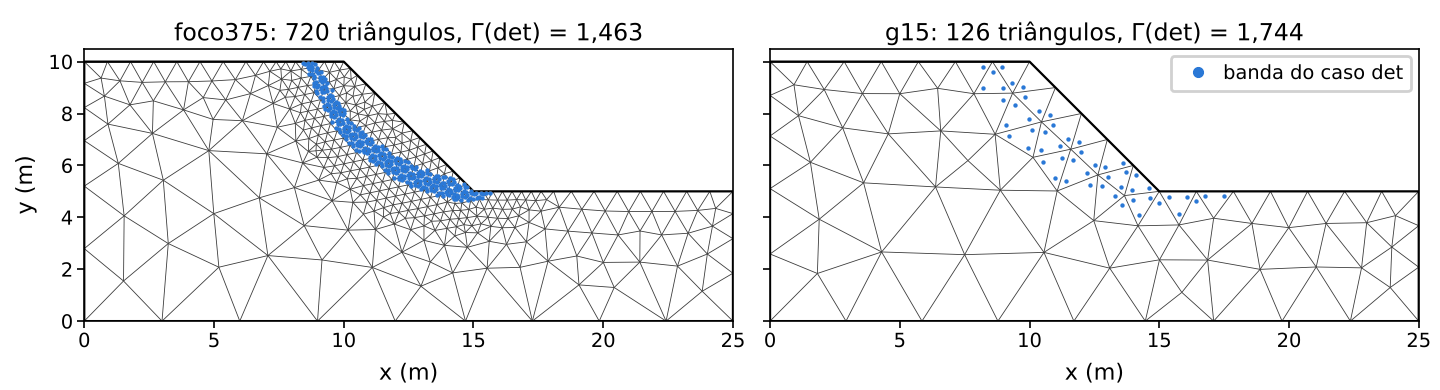
\includegraphics[width=\textwidth]{figuras/niv_malhas_iniciais.png}
  \caption{Malhas iniciais (etapa~1) do estudo de níveis: foco375 (720 triângulos; $h = 0{,}375$~m
    na faixa em torno das bandas de um estudo anterior, Figura~\ref{fig:ref:malhas_fixas}) e g15
    (126 triângulos; o mesmo contorno sem o foco, só com 1,5~m perto da superfície e até 3~m no
    interior). Em azul, a banda de ruptura do caso determinístico obtida em cada uma (pontos de
    integração com $\sqrt{J_2}$ da deformação plástica $\geq 0{,}1$ do máximo no instante do fator),
    que guia o refino; $\Gamma(\mathrm{det}) = 1{,}463$ na foco375 e $1{,}744$ na g15.}
  \label{fig:niv:malhas_iniciais}
\end{figure}

\begin{figure}[htbp]
  \centering
  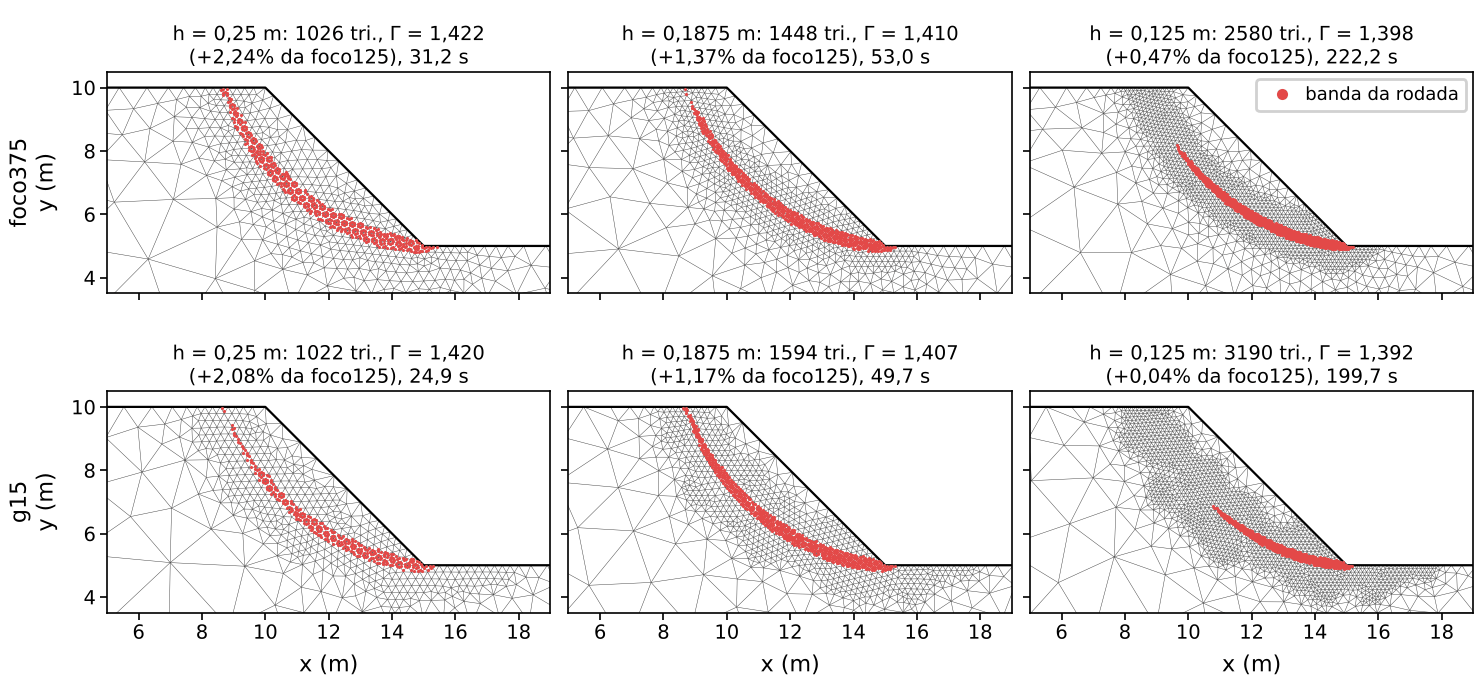
\includegraphics[width=\textwidth]{figuras/niv_niveis_det.png}
  \caption{Níveis de refinamento num passo, caso determinístico. Linhas: malha inicial (foco375,
    g15); colunas: tamanho $h$ dos elementos em torno da banda da etapa~1 (0,25, 0,1875 e
    0,125~m, sempre até 0,375~m dos pontos da banda). Cada painel mostra a malha refinada,
    ampliada na região do talude, e a banda da sua rodada (em vermelho, mesma definição da
    Figura~\ref{fig:niv:malhas_iniciais}). Títulos: triângulos, $\Gamma$, diferença relativa ao
    $\Gamma$ da malha fixa foco125 ($1{,}391$) e tempo de CPU da cadeia (etapa~1 + geração da
    malha + rodada refinada). Na foco375, a coluna $h = 0{,}125$~m é a malha refinada da comparação
    (Figura~\ref{fig:ref:metodo_det}), rodada com 2 processos simultâneos (3 no estudo de níveis).}
  \label{fig:niv:niveis_det}
\end{figure}

\begin{figure}[htbp]
  \centering
  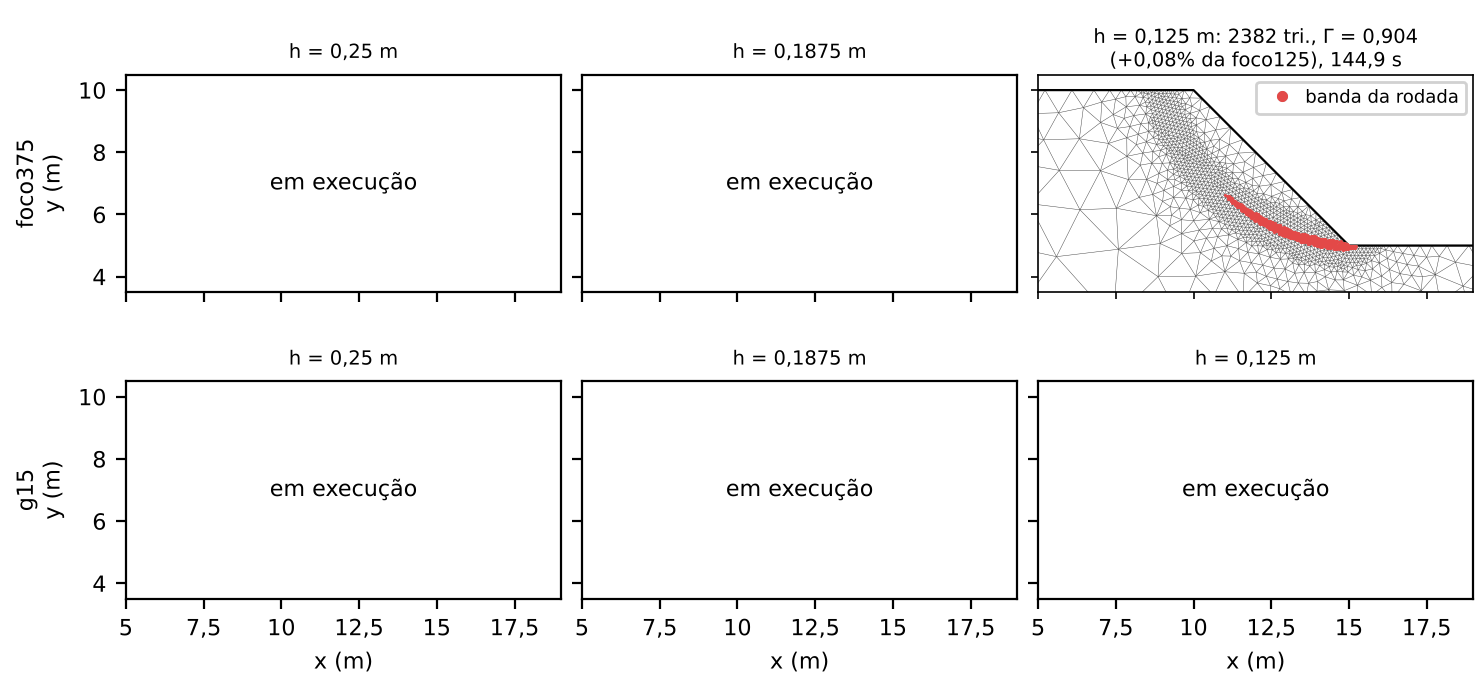
\includegraphics[width=\textwidth]{figuras/niv_niveis_r00005.png}
  \caption{Como na Figura~\ref{fig:niv:niveis_det}, para a realização r5, a de menor $\Gamma$
    ($0{,}903$ na foco125).}
  \label{fig:niv:niveis_r5}
\end{figure}

\begin{figure}[htbp]
  \centering
  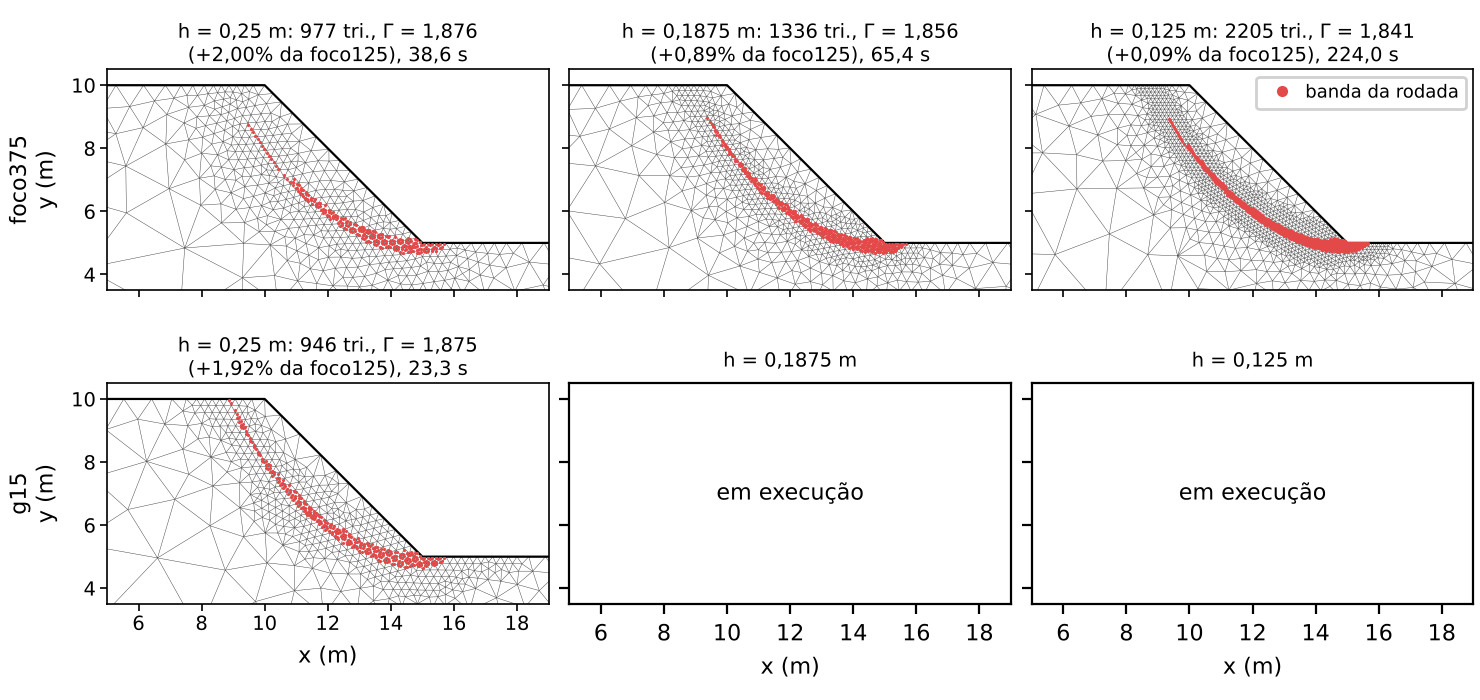
\includegraphics[width=\textwidth]{figuras/niv_niveis_r00003.png}
  \caption{Como na Figura~\ref{fig:niv:niveis_det}, para a realização r3, a de maior $\Gamma$
    ($1{,}840$ na foco125).}
  \label{fig:niv:niveis_r3}
\end{figure}

\begin{figure}[htbp]
  \centering
  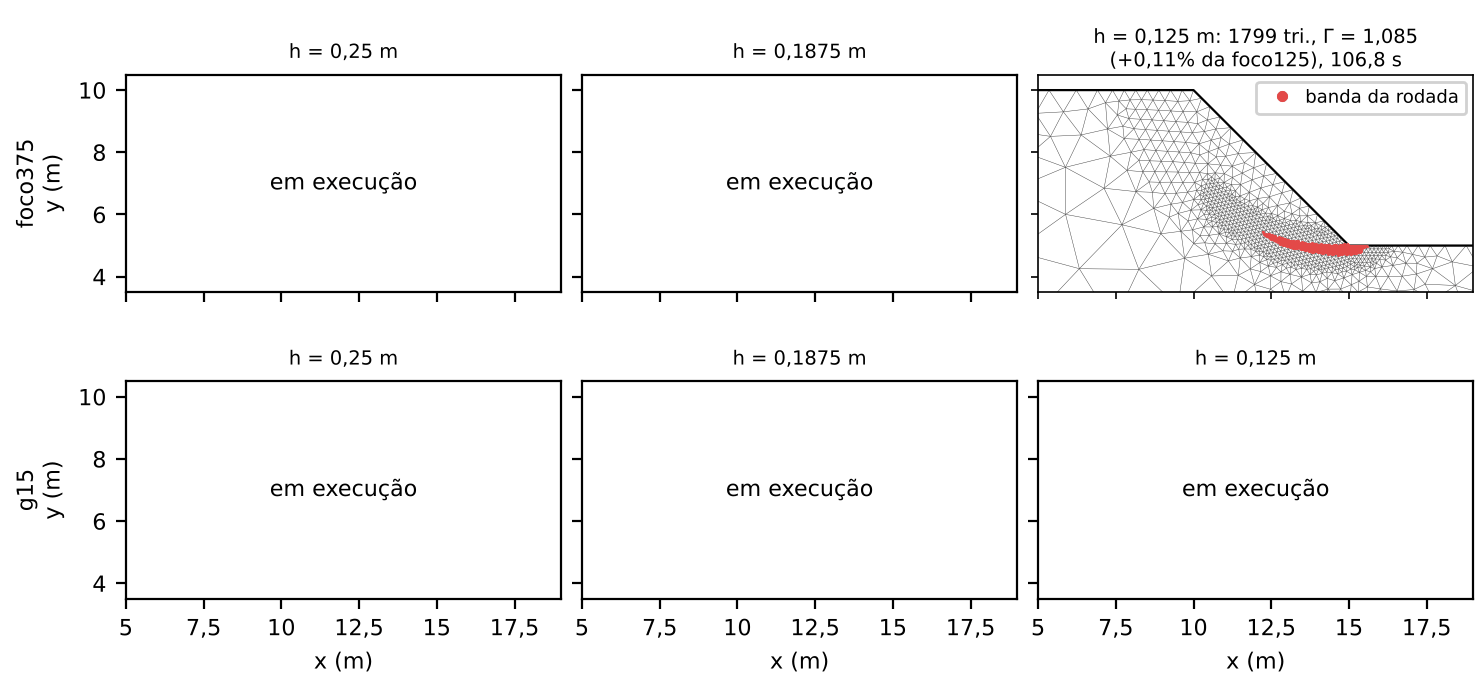
\includegraphics[width=\textwidth]{figuras/niv_niveis_r00007.png}
  \caption{Como na Figura~\ref{fig:niv:niveis_det}, para a realização r7 ($\Gamma = 1{,}084$ na
    foco125), cuja banda fica junto ao pé do talude.}
  \label{fig:niv:niveis_r7}
\end{figure}
